% Beta Version distributed 2022.12.11 
% Updated 2022.12.19 - Font sizes for the preliminary pages were updated    
% Special thanks to S.J. Kim
% LaTex template을 제작해 준 김선중 대학원생에게 깊은 감사의 마음을 전합니다. 

\documentclass[11pt]{report}
\usepackage{geometry, graphicx, kotex, imakeidx, titlesec, array} % necessary packages
\usepackage{mathptmx}   
\usepackage{amsmath, amsthm, amssymb, mathrsfs, multirow, verbatim} % supplementary packages
\usepackage[nobiblatex]{xurl} % enable linebreak of \url command
\usepackage{indentfirst} % force indentation at every first paragraph of chapters, sections and subsections
\usepackage{booktabs} % table tool
\usepackage{ragged2e}
\usepackage{setspace}

\geometry{paper=b5paper, left=30mm, right=30mm, top=30mm, bottom=30mm} % set the paper size and the margins
  
\titleformat{\chapter}{\normalfont\huge\bfseries}{\chaptertitlename\ \thechapter.}{20pt}{\huge} % chapter style
\newtheorem{theorem}{Theorem} % theorem environment
\newtheorem{definition}{Definition} % definition environment
% if you need similar environments like lemma, corollary or remark, add them all.
\newtheorem{lemma}{Lemma} % lemma environment
\newtheorem{proposition}{Proposition} % proposition environment
\makeindex % command for making an index chapter

\linespread{1.25} % set the vertical spacing between successive lines (the ratio of the maximal height of a normal font and the base lineskip)

\renewcommand\arraystretch{1.3} % increase the vertical spacing by 30%

%%% stands for a new chapter or a new page
%% stands for a new section
% stands for a comment

% 직접 추가한 코드
\renewcommand{\theequation}{\thesection.\arabic{equation}} 

\newcommand\bs[1]{\ensuremath{\boldsymbol{#1}}}
\newcommand\bx{\ensuremath{\boldsymbol x}}
\newcommand\by{\ensuremath{\boldsymbol y}}
\newcommand\bb{\ensuremath{\boldsymbol b}}
\newcommand\bv{\ensuremath{\boldsymbol v}}
\newcommand\lip{\ensuremath{\text{Lip}}}
\newcommand\pa[2]{\ensuremath{\frac{\partial #1}{\partial #2}}}
\newcommand\norm[1]{\ensuremath{\left|\left|#1\right|\right|}}

\usepackage{booktabs,enumitem}
\renewcommand{\labelenumi}{(\roman{enumi})}

\usepackage[linesnumbered,boxed,commentsnumbered]{algorithm2e}

%%%%
\begin{document}
%%% cover page for the master's thesis
% For the doctoral degree, delete this page and use the next page

\newpage   
\begin{center}
\pagenumbering{gobble} % Cover page, title page and signature page) should not be numbered.
{\fontsize{16pt}{16pt}\selectfont Master's Thesis \par}  
\vspace{3cm} % 3cm spacing
\huge Lipschitz Constants of Neural Networks
\par\vspace{4.5cm} % spacing can be adjusted
{\fontsize{16pt}{16pt}\selectfont Sunjoong Kim \par}  % put the student's name here
\vspace{0.5cm}
{\fontsize{16pt}{16pt}\selectfont Department of Mathematics \par}  % You can reduce the character spacing to make the department name on one line. If it takes up more than two lines, please reduce the vertical spacing after the title appropriately.
\vspace{1.5cm}
{\fontsize{18pt}{18pt}\selectfont Graduate School \par} 
\vspace{0.5cm}
{\fontsize{18pt}{18pt}\selectfont Korea University \par} 
\vspace{1cm}
{\fontsize{14pt}{14pt}\selectfont February 2024} 
\end{center}

%%% title page for master's thesis
% For the doctoral degree, delete this page and use the next page
\newpage 
\begin{center}
\huge Lipschitz Constants of Neural Networks
\par\vspace{3.1cm} % spacing can be adjusted
{\fontsize{16pt}{16pt}\selectfont by \par Sunjoong Kim \par}
\vspace{0.5cm}
\rule{.6\textwidth}{0.4pt} %  % Student signature is required above the line
\par\vspace{0.2cm}
{\fontsize{16pt}{16pt}\selectfont under the supervision of Professor Seungsang Oh \par}
\vspace{0.7cm}
{\fontsize{16pt}{18pt}\selectfont A thesis submitted in partial fulfillment of \par
 the requirements for the degree of \par Master of Mathematics \par }   
\vspace{10pt}
{\fontsize{16pt}{16pt}\selectfont Department of Mathematics} % You can reduce the character spacing to make the department name on one line. If it takes up more than two lines, please reduce the vertical spacing after the title appropriately.
\par\vspace{1.5cm}
{\fontsize{18pt}{18pt}\selectfont Graduate School \par \vspace{0.5cm}
 Korea University \par} 
\vspace{1cm}
{\fontsize{14pt}{14pt}\selectfont October 2023} % month and year of the submission deadline for the thesis/dissertation examination copy.
\end{center}

%%% signature page for the master's degree
% For the doctoral degree, delete this page and use the next page

\newpage 
\begin{center}
\vspace{1cm}
{\fontsize{16pt}{18pt}\selectfont
The thesis of Sunjoong Kim has been approved \par
by the thesis committee in partial fulfillment\par
of the requirements for the degree of \par
Master of Mathematics \par}  
\vspace{1cm}
{\fontsize{14pt}{14pt}\selectfont December 2023} % the year and month of including the date the thesis examination was completed 
\par\vspace{3cm}
\rule{.6\textwidth}{0.4pt}\par % committee's signature above the line 
{\fontsize{16pt}{16pt}\selectfont Committee Chair: Name \par} %%%%% 수정필요 : 교수님 성함?
\vspace{1cm}
\rule{.6\textwidth}{0.4pt}\par % committee's signature above the line 
{\fontsize{16pt}{16pt}\selectfont Committee Member: Name \par}
\vspace{1cm}
\rule{.6\textwidth}{0.4pt}\par % committee's signature above the line 
{\fontsize{16pt}{16pt}\selectfont Committee Member: Name \par}
\end{center}

%%% English abstract page
\newpage 
\pagenumbering{roman} % set the page number as roman type from this page on.
\newgeometry{paper=b5paper, left=20mm, right=20mm, top=30mm, bottom=30mm} % set the paper size and the margins
% Margins shall be changed to bottom and top 3 cm, right and left 2 cm from this page forward.
\addcontentsline{toc}{chapter}{Abstract}
\begin{center}
\LARGE Lipschitz Constants of Neural Networks % put the title here
\par\vspace{20pt}

\normalsize \doublespacing
by Sunjoong Kim\par % put the student name here
Department of Mathematics\par
under the supervision of Professor Seungsang Oh % put the professor's name and the department here
\par\vspace{20pt}
\large \textbf{Abstract}
\end{center}

\normalsize
\justifying % this command available with \usepackage{ragged2e}
\doublespacing

In machine learning and deep learning, making an algorithm stable or robust is just as important as making it perform well.
One of the indicator that measures the sensitiveness or the robustness of an algorithm is the Lipschitz constant.
This paper discusses several ways to calculate the Lipschitz constant of basic machine learning algorithms.
One of the  main part of the perceptron and MLP is the linear function, whose Lipschitz constant coincide with the operator norm of the corresponding matrix.
Unlike the linear function, evaluating the optimal Lipschitz constant of many algorithms is difficult or infeasible even for the two layered MLP.
Instead of calculating the exact constant, there is a systematic way called \emph{AutoLip} to find an upper bound for the constant and we apply it to MLP and CNN.
For example, the convolution layer can be thought of as a matrix multiplication by a long matrix and it may require several tools to make it simple.

\par\vspace{20pt}
\textbf{Keywords}: Lipschitz constant, Operator norm, Rademacher's theorem, AutoLip, Power method, Rayleigh quotient

%%% Korean abstract page

\newpage 
\begin{center}
\LARGE 인공신경망의 립시츠 상수 % put the title here
\par\vspace{20pt}
\normalsize 김 선 중\par % put the student name here
수 학 과\par % put the professor's name and the department here
지 도 교 수:  오 승 상
\par\vspace{20pt}
\addcontentsline{toc}{chapter}{국문초록}
\large \textbf{국문 초록}
\end{center}

\normalsize 

머신러닝과 딥러닝에서 안정적인 알고리즘을 만드는 것은 그 알고리즘이 좋은 성능을 내는 것 만큼이나 중요하다.
알고리즘의 안정성과 관련되어 있는 수학적인 개념 중 하나는 립시츠 상수이다.
이 논문에서는 기본적인 머신러닝 알고리즘의 립시츠 상수를 계산하는 다양한 방법에 대해 논의한다.
가장 기본적인 구조인 퍼셉트론은 선형함수의 구조를 가지고 있고, 선형함수의 립시츠 상수는 그 선형함수에 대응되는 행렬에 대한 작용소 놈의 값과 일치한다.
하지만, 선형함수에서 조금만 알고리즘이 복잡해져도 립시츠 상수를 계산하는 것은 어려워진다.
예를들어, 레이어가 두 개인 다층퍼셉트론의 경우만 해도 정확하게 립시츠 상수를 계산하는 것이 거의 불가능하다(NP-hard).
그래서 이 논문에서는, 다양한 머신러닝 알고리즘의 정확한 립시츠 상수값을 계산하는 대신 립시츠 상수의 상한(upper bound)을 계산하는 체계적인 알고리즘(AutoLip)을 소개하고, 이것을 다층퍼셉트론과 합성곱신경망에 적용해본다.
합성곱 레이어는, 특정한 형태의 행렬의 행렬곱으로 이해할 수 있고, 따라서 작용소 놈을 계산하면 립시츠 상수가 얻어진다.
이때, 효율적인 계산을 위해 누승법이나 레일리몫과 같은 방법이 사용될 수 있다.

\par \vspace{20pt}
\textbf{중심어} : 립시츠 상수, 작용소 놈, Rademacher 정리, AutoLip, 누승법, 레일리 몫

%%% dedication : 생략

%%% preface : 생략

%\newpage
%\chapter*{Preface}
%\addcontentsline{toc}{chapter}{Preface}
%\normalsize
%The text of the preface begins here. 
%
%If the thesis/dissertation contains the results of work conducted in collaboration with other people, or if the thesis/dissertation contains previously published content, a preface must be included. The preface may include the following. However, it is also possible to include the contents of the preface in the introduction of the main body.\par
%
%\begin{enumerate}
%\item a description of the results that were obtained in collaboration with others, indicating the nature and proportion of the contribution of others and in general terms the portions of the work which the student claims as original 
%\item acknowledgments of funding sources and other contributors
%\item a description of contents that have been \underline{published or submitted for publication} and the contributions of all authors involved in any multi-authored publications included in the thesis/dissertation 
%\item your brief personal background, academic motivation, thesis/dissertation target group, acknowledgments, etc. can be included 
%\end{enumerate}
%
%\newpage
%Examples you may refer to 
%\begin{itemize}
%\item\url{https://www.grad.ubc.ca/sites/default/files/doc/page/thesis_sample_prefaces.pdf}
%\item\url{https://www.phase-trans.msm.cam.ac.uk/2002/thomas/chapter1.pdf}
%\end{itemize}

%%% acknowledgment : 생략

%%% table of contents
\renewcommand*\contentsname{Table of Contents}
\addcontentsline{toc}{chapter}{Table of Contents}
\tableofcontents

\bigskip

%The table of contents starts with the abstract. 
%The preliminary pages (abstract, dedication, preface, acknowledgments, table of contents, list of tables, list of figures, nomenclature) should be assigned using small Roman numerals (i, ii, iii, iv, v...). The other preliminary pages (cover page, title page, and signature page) should not be numbered. For the main body, use Arabic numbers (1, 2, 3, 4, 5...) starting with page 1.
%It is customary to use Arabic numbers (1, 2, 3, 4, 5...) for the chapters in the main body and capital letters (A, B, C...) for the sections in the appendices.

%%% list of tables
\listoftables
\addcontentsline{toc}{chapter}{List of Tables}

\bigskip
%A list of tables shall be included when there are tables in the thesis/dissertation. Table numbering can be continuous throughout the thesis/dissertation or by chapter (e.g., 1.1, 1.2, 2.1, 2.2...).

%%% list of figures
\listoffigures
\addcontentsline{toc}{chapter}{List of Figures}

\bigskip
%List of figures should be prepared when figures are included in the thesis/dissertation. Figure numbering can be continuous throughout the thesis/dissertation or by chapter (e.g., 1.1, 1.2, 2.1, 2.2...).

%%%% nomenclature (or list of symbols) 
%\chapter*{Nomenclature}
%\addcontentsline{toc}{chapter}{Nomenclature}
%\begin{tabular}{p{.2\textwidth}p{.7\textwidth}}
%$M$	& original mass matrix\\
%$K$	& original stiffness matrix\\[30pt]
%\multicolumn{2}{l}{Subscripts}\\
%$b$ & interface boundary\\
%$d$ & dominant\\[30pt]
%\multicolumn{2}{l}{Abbreviation}\\
%$CMS$ & Component Mode Synthesis\\
%\end{tabular}
%
%\bigskip
%If nomenclature or a list of symbols is used, a section describing subscripts and abbreviations can be included.

%%% first chapter of the main body

\chapter{Introduction}\label{chap:intro}
\pagenumbering{arabic} % set the page number as Arabic type from this page on.

Deep neural networks have made many advances including computer vision, language modeling, machine translation and text and picture generating.
Still, one of the difficulties in applying deep learning algorithms to reality is that the algorithm often lacks its robustness.
As an example, Szegedy et al. have found that a small perturbation of an input for true image may cause the classifier to misclasssify the image as false image \cite{CS-WZ}.

To overcome the instabiltiy of training and to enhance robustness of generating models such as GANs, M. Arjovsky et al. proposed Wasserstein distance between distributions and restrict their attention to 1-Lipschitz function to the critic \cite{MA-SC}, \cite{GI-AF}.
As this example suggest, the Lipschitz constant can be a good metric to access the robustness of the algorithm.

The Lipschitz constant of a function measures the sensitiveness or the robustness, or the rate of changes of the function.
In chapter 2, we define the optimal Lipschitz constant of the functions between euclidean spaces and explore the computation of this optimal constant for various functions including linear maps, affine maps and compositions of functions.
However, if the function becomes more complex, it is difficult or almost impossible to calculate the optimal constant.
So, we propose algorithms to estimate the constant, using the Rademacher's theorem.

%%%  the second chapter of the main body
%%%
\chapter{Lipschitz Constants of Functions Between Euclidean Spaces}

%%
\section{Lipschitz Constants}
% Definition : A Liptschitz constant (LC) and The optimal Lipschitz constant(OLC), extension to the metric space functions
%Let \(f:\mathbb R^n\to\mathbb R^m\) be a function.
For vectors \(\bx=[x_1\:\:\cdots\:\:x_n]^T\) and \(\by=[y_1\:\:\cdots\:\:y_m]^T\) in Euclidean spaces \(\mathbb R^n\) and \(\mathbb R^m\), respectively, \(||\bx||\) and \(||\by||\) are the usual standard norms of \bx{} and \by{} defined by
\begin{equation}\label{eq:euclidean_norm}
||x||=\sqrt{{x_1}^2+\cdots+{x_n}^2},\quad ||y||=\sqrt{{y_1}^2+\cdots+{y_m}^2}.
\end{equation}

\begin{definition}\label{LC}
A function \(f:\mathbb R^n\to\mathbb R^m\) is called \emph{Lipschitz continuous} if there is a nonnegative real number \(c\) such that
\begin{equation}\label{eq:LC1}
||f(\bx)-f(\by)||\le c||\bx-\by||\qquad(\bx,\by\in\mathbb R^n)
\end{equation}
The infimum of \(c\) which satisfies \eqref{eq:LC1} is called the \emph{Lipschitz constant} of \(f\) and is denoted by \(\lip(f)\).
%If \(\lip(f)\) exists as a nonnegative real number, \(f\) is called a Lipschitz continuous function.
\end{definition}

% The equality of inf-def and sup-def
This definition can also be extended to functions from a metric space to another metric space if we substitute the norms with the distances.
It is useful to know that there is an equivalent definition ;
\begin{equation}\label{eq:LC2}
\lip(f)=\sup_{\bx\neq\by}\frac{||f(\bx)-f(\by)||}{||\bx-\by||}
\end{equation}
To show the equivalence of the two definitions, let
\begin{equation}\label{eq:equivalent_def}
\begin{aligned}
L_1&=\inf\{c\ge0:||f(\bx)-f(\by)||\le c||\bx-\by||,\quad\bx,\by\in\mathbb R^n\}\\
L_2&=\sup\left\{\frac{||f(\bx)-f(\by)||}{||\bx-\by||}:\bx,\by\in\mathbb R^n,\bx\neq\by\right\}.
\end{aligned}
\end{equation}
Let \(\mathcal L_1\) and \(\mathcal L_2\) be two the sets in the definition of \(L_1\) and \(L_2\), respectively.
Then, \(\mathcal L_2\subset\mathcal L_1\) since
\[\mathcal L_2=\{c\ge0:||f(\bx)-f(\by)||=c||\bx-\by||,\quad\bx,\by\in\mathbb R^n,\bx\neq\by\},\]
and it follows that \(L_1\le L_2\).
%Pick \(c\in\mathcal L_2\).
%Then, \(c\in\mathcal L_1\) and it follows that \(L_1=\inf\mathcal L_1\le c\).
%Since \(c\in\mathcal L_2\) was arbitrary, we can take supremum for all \(c\in\mathcal L_2\) to conclude that \(L_1\le L_2\).
Pick \(c\in\mathcal L_1\).
Then, \(||f(\bx)-f(\by)||\le c||\bx-\by||\) for all \(\bx\) and \(\by\) in \(\mathbb R^n\).
Assuming \(\bx\neq \by\), we have
\[
\frac{||f(\bx)-f(\by)||}{||\bx-\by||}\le c.
\]
Taking supremum for all \bx{} and \by{} (\(\bx\neq\by\)), we have \(L_2\le c.\) and taking infimum for all \(c\le\mathcal L_1\) yields \(L_2\le L_1\).
Thus the two definitions are indeed equivalent.

% inf = min
The optimal Lipschitz constant \(\lip(f)\) is not only the infimum, but also the minimum of \(L\) satisfying \eqref{eq:LC1}.
To show this, it suffices to prove that \(\lip(f)\in\mathcal L_1\), or that \(c=\lip(f)\) satisfies the condition.
Let \(\bx,\:\by\in\mathbb R^n\).
If \(\bx=\by\), then \eqref{eq:LC1} holds trivially.
Assuming \(\bx\neq\by\), we have
\[
\frac{||f(\bx)-f(\by)||}{||\bx-\by||}\le\lip(f)
\]
because of the second definition \eqref{eq:LC2} of \(\lip(f)\).
Multiplying both sides by \(||\bx-\by||\), we can conclude that \(c=\lip(f)\) satisfies the condition \eqref{eq:LC1}.
% sup = max도 증명하면 좋겠는데, 어떻게 해야 할 지 모르겠다.
% f가 linear map인 경우에는 conrad의 방법을 사용하면 된다.
% conrad의 방법을 여기에 쓰자니, 가능은 할 것 같은데 말이 너무 길어지는 것 같다.

% lip=0 iff constant function
Note also that \(\lip(f)=0\) if and only if \(f\) is a constant function.
Suppose that \(f\) is a constant function.
Then, the condition \eqref{eq:LC1} holds vacuously and \(\mathcal L_1=[0,\infty)\) ; \(\lip(f)=0\).
Suppose, on the contrary, that \(\lip(f)=0\).
Pick \(\bx,\by\in\mathbb R^n\).
Since \(0\in\mathcal L_1\), we have \(||f(\bx)-f(\by)||=0\).
Thus, \(f(\bx)=f(\by)\) and \(f\) is a constant function.
% Finding OLC is NP-hard [1]

%%
\section{Real-valued Functions of a Real Variable}
% Average rate of change
% differentiable (almost) everywhere → mean value theorem
% sigmoid, hyperbolic tangent, ReLU

For univariate real function \(f:\mathbb R\to\mathbb R\), the above condition \eqref{eq:LC1} is equivalent to saying that the average rate of change is upper bounded by \(c\);
\begin{equation}\label{eq:LC_average_rate_of_change}
\left|\frac{f(x)-f(y)}{x-y}\right|\le c.
\end{equation}
If \(f\) is diffrentiable everywhere in the domain, the mean value theorem guarantees that this is equivalent to 
\begin{equation}\label{eq:LC_univariate1}
|f'(x)|\le c
\end{equation}
for every \(x\in\mathbb R\).
Moreover, \(\lip(f)\) is the least nonnegative number \(c\) satisfying the condition \eqref{eq:LC_univariate1} for all \(x\) and we can express \(\lip(f)\) in its exact form ; 
\begin{equation}\label{eq:LC_univariate2}
\lip (f) = \sup_{x\in\mathbb R}|f'(x)|
\end{equation}

In this sense, we can easily evaluate the optimal Lipschitz constant of the sigmoid function
\begin{equation}\label{eq:sigmoid}
\sigma(x)=\frac1{1+e^{-x}}
\end{equation}
and the hyperbolic tangent function
\begin{equation}\label{eq:tanh}
\tanh(x)=\frac{e^x-e^{-x}}{e^x+e^{-x}}.
\end{equation}
Since \(0<\sigma(x)<1\) and \(\sigma'(x)=\sigma(x)\left(1-\sigma(x)\right)\), we have \(\sigma'(x)<\frac14\) so that
\begin{equation}\label{eq:sigmoid_LC}
\lip(\sigma)=\frac14.
\end{equation}
Since \(\tanh(x)=2\sigma(2x)-1\), we have
\[\tanh'(x)=4\sigma'(2x)<1\]
and
\begin{equation}\label{eq:tanh_LC}
\lip(\tanh)=1.
\end{equation}

The \text{ReLU} function
\begin{equation}\label{eq:ReLU}
\text{ReLU}(x)=\max\{0,x\}
\end{equation}
 is not differentiable everywhere, but we can use \eqref{eq:LC_average_rate_of_change} to conclude
\begin{equation}\label{eq:ReLU_LC}
\lip(\text{ReLU})=1.
\end{equation}
%Although not being differentiable, the case of rectified linear unit \(\text{ReLu}(x)=\max\{0,x\}\) can also be easily evaluated to be \(1\).
Here is a list of the optimal Lipschitz constants of univariate activation functions, frequently used in machine learning and deep learning. (\textbf{Table} \ref{tab:univariate_activation_functions})
 
\renewcommand\arraystretch{1.5}
\begin{table}[ht]
\centering
\caption{The Lipschitz constants of univariate activation functions.}
\label{tab:univariate_activation_functions}
%\(\alpha=0.1\) for Leaky ReLU and \(\alpha=1\) for ELU.
\begin{tabular}[t]{llc}
\toprule
Activation Functions	&Formula									& $\lip(f)$\\
\midrule
Sigmoid				&$\sigma(x)=\frac1{1+e^{-x}}$				&$\frac14$\\
Hyperbolic tangent	&$\tanh(x)=\frac{e^x-e^{-x}}{e^x+e^{-x}}$	&1\\
Rectified Linear Unit	&$\text{ReLU}(x)=\max\{0,x\}$			&1\\
Leaky ReLU			&$\text{LReLU}(x)=\max\{\alpha x,x\}$	&1\\
Exponential Linear Unit&$\text{ELU}(x)=
\begin{cases}x&(x\ge0)\\\alpha(e^x-1)&(x<0)\end{cases}$	&1\\
Softplus			&$f(x)=\frac1\beta\log(1+e^{\beta x})$	&$1$\\
Gaussian			&$g(x)=e^{-x^2}$								&$\sqrt{\frac2e}$\\
\bottomrule
\end{tabular}
\end{table}

In the definition of \(\lip(f)\) in \eqref{eq:LC2}, we can't replace the supremum by the maximum.
Consider a function ; \(f(x)=\ln(1+e^x)\).
This function is called the softplus activation function and is an antiderivative of the sigmoid function.
It is a monotonically increasing function whose derivative is also increasing, with an assymptote \(y=x\).
Thus, \(\lip(f)=1\), but no \(x\) and \(y\) satisfy the equality \(\frac{f(x)-f(y)}{x-y}=1\).

%%
\section{Linear Functions}
% Operator norms of matrices matches the notion of OLC

%
\subsection{Operator Norms \(||W||\)}

Consider a linear function \(f(\bx)=W\bx\) for some \(m\times n\) matrix \(W\).
Because of the linearity, the condition \eqref{eq:LC1} reduces to
\begin{equation}\label{eq:linear_LC}
||W\bx||\le c||\bx||.\qquad(\bx\in\mathbb R^n)
\end{equation}

The smallest \(c\) which satisfies \eqref{eq:linear_LC} is called \emph{the operator norm of \(W\)} and denoted by \(||W||\).
Thus, the optimal Lipschitz constant of \(f\) equals the operator norm of \(W\) ; \(||W||=\lip(f)\).
The definitions of the forms \eqref{eq:equivalent_def} are as follows;
\begin{equation}\label{eq:linear_equivalent_def}\begin{aligned}
||W||
&=\inf\left\{c\ge0\::\: ||W\bx||\le c||\bx||\right\}\\
&=\sup\left\{\frac{||W\bx||}{||\bx||}\;:\;\bx\in\mathbb R^n,\:\bx\neq\bs0\right\}
\end{aligned}\end{equation}
If we modify the second definition of \eqref{eq:linear_equivalent_def} to
\begin{equation}\label{eq:linear_equivalent_def_2}
||W||=\sup\left\{||W\bx||:||\bx||=1\right\},
\end{equation}
we can easily verify that the supremum is actually the maximum in this case.
Because the set \(\{\bx:||\bx||=1\}\) is a compact subset of \(\mathbb R^n\) and the map \(\bx\mapsto||W\bx||\) is continuous, the set in \eqref{eq:linear_equivalent_def_2} has its maximum.

The operator norm is indeed a norm of a vector space ;
\begin{proposition}\label{prop:operator_norm_1}
The operator \(||\cdot||:W\mapsto||W||\) satisfies the following three properties.
Thus, the set \(\mathcal M_{m,n}(\mathbb R)\) of all \(m\) by \(n\) real matrices is a normed vector space with respect to this norm ;
\begin{enumerate}[label=(\alph*)]
\item
\(||W||\ge0\) for all \(W\in\mathcal M_{m,n}(\mathbb R)\) ; \(||W||=0\) if and only if \(W=0\).
\item
\(||kW||=|k|\cdot||W||\) for all \(W\in\mathcal M_{m,n}(\mathbb R)\) and \(k\in\mathbb R\).
\item
\(||W+V||\le||W||+||V||\) for all \(W,V\in\mathcal M_{m,n}(\mathbb R)\).
\end{enumerate}
\end{proposition}
For (a), that \(||W||\ge0\) is obvious.
If \(||W||=0\), then \(||W\bx||\le 0||\bx||=0\) for all \(\bx\in\mathbb R^n\).
It follows that \(W\bx=0\) for all \(\bx\in\mathbb R^n\), by the definition of vector norm, thus \(W=0\).
Suppose, on the other hand, that \(W=0\). Then \(W\bx=0\) for all \(x\in\mathbb R^n\).
Thus, \(c=0\) is the minimal value satisfying \eqref{eq:linear_LC}.
To prove (b), we have
\begin{align*}
||kW||
&=\inf\left\{c:||kWx||\le c||x||\right\}\\
&=\inf\left\{c:|k|\cdot||Wx||\le c||x||\right\}\\
&=\inf\left\{c:||Wx||\le\frac{c}{|k|}||x||\right\}\\
&=\inf\left\{|k|b:||Wx||\le b||x||\right\}\\
&=|k|\inf\left\{b:||Wx||\le b||x||\right\}\\
&=|k|\cdot||W||.
\end{align*}
Now, consider (c).
For any \(\bx\in\mathbb R^n\), we have
\begin{align*}
||(W+V)\bx||
&=||W\bx+V\bx||\le||W\bx||+||V\bx||\\
&\le||W||\:||\bx||+||V||\:||\bx||=(||W||+||V||)||\bx||
\end{align*}
By the minimality of \(||W+V||\), we have \(||W+V||\le||W||+||V||\).

An analogue of (c) also holds for multiplication;
if \(W\in\mathcal M_{m,n}(\mathbb R)\) and \(V\in\mathcal M_{n,k}(\mathbb R)\), then
\begin{equation}\label{eq:multiplicative_inequality}
||WV||\le||W||\:||V||.
\end{equation}
This is because of the inequality
\[||(WV)\bx||=||W(V\bx)||\le||W||\:||V\bx||\le||W||\:||V||\:||\bx||\]
and the minimality of \(||WV||\).

%
\subsection{Evaluation of \(||W||\) for square matrices}

First, consider the case when \(W\) is a square matrix so that \(f:\mathbb R^n\to\mathbb R^n\).
Let \(\lambda_1\), \(\cdots\), \(\lambda_n\) be (possibly repeated) eigenvalues of \(W\) and let \(\tilde\lambda=\max\{|\lambda_i|\::\:i=1,\cdots,n\}\).
(\(\tilde\lambda\) is sometimes called the \emph{dominating eigenvalue}, especially in the context of the power method : Subsection \ref{sec:power_method})
Then, the following inequality holds in general ;
\begin{equation}\label{eq:square_matrix_inequality_1}
\tilde\lambda\le||W||.
\end{equation}
For a proof, pick an eigenvalue \(\lambda_i\) and the corresponding eigenvector \(\bx_i\) which is nonzero.
Since \(W\bx_i=\lambda_i\bx_i\),
Then, we have \(||W\bx_i||=|\lambda_i|\:||\bx_i||\) and
\[|\lambda_i|=\frac{||W\bx_i||}{||\bx_i||}\le||W||.\]
Taking the maximum over \(i\), we have the desired inequality.
The above inequality \eqref{eq:square_matrix_inequality_1} becomes equality when \(W\) is symmetric.

Suppose that \(W\) is real symmetric.
Then, \(W\) is orthogonally diagonalizable in the sense that, there exists an orthogonal matrix
\[V=[\bv_1\quad \cdots \quad \bv_n],\]
%which is orthogonal (and thus \(\{\bv_1,\cdots,\bv_n\}\) is orthonormal.)
such that
\[W=V\Lambda V^T,\]
where \(\Lambda=\text{diag}\{\lambda_1,\cdots,\lambda_n\}\) and \(\lambda_i\) is an eigenvalue of \(W\) with the corresponding eigenvector \(\bv_i\).
Note that \(\{\bv_1,\cdots,\bv_n\}\) forms an orthonormal basis for \(\mathbb R^n\).
For any nonzero \(\bx\in\mathbb R^n\), there exist real numbers \(c_1\), \(\cdots\), \(c_n\) such that \(\bx=c_1\bv_1+\cdots+c_n\bv_n\).
Since
\begin{align*}
W\bx
&=c_1W\bv_1+\cdots+c_nW\bv_n\\
&=c_1\lambda_1\bv_1+\cdots+c_n\lambda_n\bv_n,
\end{align*}
we have (by the orthogonality of \(v_i\)'s
\begin{align*}
||W\bx||^2
&=||c_1W\bv_1+\cdots+c_nW\bv_n||^2\\
&=|c_1\lambda_1|^2||\bv_1||^2+\cdots+|c_n\lambda_n|^2||\bv_n||^2\\
&={c_1}^2{\lambda_1}^2+\cdots+{c_n}^2{\lambda_n}^2.
\end{align*}
Thus,
\[\frac{||W\bx||^2}{||\bx||^2}=\frac{{c_1}^2{\lambda_1}^2+\cdots+{c_n}^2{\lambda_n}^2}{{c_1}^2+\cdots+{c_n}^2}
\le{\tilde\lambda}^2,\]
for which \(||W\bx||/||\bx||\le\tilde\lambda\).
Therefore, we have the reverse inequality \(||W||\le\tilde\lambda\).

As examples consider the following matrices \(W_1\), \(W_2\), \(W_3\), \(W_4\), \(W_5\) defined by
\begin{gather*}
W_1=\begin{bmatrix}
1&0\\0&1
\end{bmatrix},\quad
W_2=\begin{bmatrix}
2&0\\0&3
\end{bmatrix},\quad
W_3=\begin{bmatrix}
4&2\\2&7
\end{bmatrix},\\
W_4=\begin{bmatrix}
1&3\\2&0
\end{bmatrix},\quad
W_5=\begin{bmatrix}
0&1\\0&0
\end{bmatrix}.\quad
\end{gather*}
\(W_1\) is the identity matrix and thus it must be that \(||W||=1\).
Indeed, the characteristic polyinomial of \(W_1\) is \((\lambda-1)^2=0\), \(\lambda_1=\lambda_2=1\) and thus the maximum absolute value of them is \(1\).
The matrix \(W_2\) stretches a given vector \(\bx\) twice in the x-axis direction and three times in the y-axis direction.
Thus, \(||W_2||\) should be \(3\).
Indeed, \(|W_2-\lambda I|=(\lambda-2)(\lambda-3)\) and \(\tilde\lambda=3\).
\(W_3\) is the last example that is symmetric ; \(|W_3-\lambda I|=(\lambda-3)(\lambda-8)\) and \(\tilde\lambda=8\).

\(W_4\) is not symmetric and we can't evaluate \(||W_4||\) for now.
Still, we have, \(\lambda_1=-2\), \(\lambda_2=3\) and \(||W_4||\ge3\) by \eqref{eq:square_matrix_inequality_1}.
The reverse inequality is not valid since the eigenvectors \(x_1=[1\:\:-1]^T\) and \(x_2=[3\:\:2]^T\) are not perpendicular.
\(W_5\) is not symmetric either, but we can postulate that \(||W_5||=1\) since
\[
W_5\bx=
\begin{bmatrix}
0&1\\0&0
\end{bmatrix}
\begin{bmatrix}
x_1\\x_2
\end{bmatrix}
=
\begin{bmatrix}
x_2\\0
\end{bmatrix}
\]
and
\[
\frac{||W_5\bx||}{||\bx||}=\frac{|x_2|}{\sqrt{{x_1}^2+{x_2}^2}}\le 1.
\]
Since \(W_5\) has the only eigenvector \(0\), the inequality \eqref{eq:square_matrix_inequality_1} still holds.

Here is a short description of what we've done in this subsection.
\begin{lemma}\label{lemm:evaluation_for_square_matrices}
Let \(W\in\mathcal M_n(\mathbb R)\) be a real symmetric matrix.
Then, the operator norm \(||W||\) is the maximal absolute eigenvalue of \(W\).
\end{lemma}

%
\subsection{Evaluation of \(||W||\) for rectangular matrices}\label{sec:evaluation_for_rectangular_matrices}
Almost all matrices that we encounter in machine learning problem are neither symmetric matrices, nor are they square matrices.
But, we can always calculate the Lipschitz constant or the operator norm of any rectangular matrices.
%Aside from the properties listed in the Proposition \ref{prop:operator_norm_1}, there is a useful criteria that help find the optimal Lipschitz constant of any rectangular matrix.

\begin{theorem}\label{theo:evaluation_for_rectangular_matrices}
\cite{KC}
Let \(W\in\mathcal M_{m,n}(\mathbb R)\) be an \(m\) by \(n\) real matrix.
Then
\begin{equation}\label{eq:evaluation_of_operator_norm_for_rectangular_matrix}
||W||=\sqrt{||W^TW||}.
\end{equation}
\end{theorem}

Note that the norm on the left hand side is the operator norm on \(\mathcal M_{m,n}(\mathbb R)\) and the norm on the right hands side is the operator norm on \(\mathcal M_n(\mathbb R)\).
Note also that the matrix \(W^TW\) is real symmetric in that \((W^TW)^T=W^T(W^T)^T=W^TW\) and we are always able to calculate the norm of \(||W^TW||\) by making use of the lemma \ref{lemm:evaluation_for_square_matrices}.

Before the proof of \eqref{eq:evaluation_of_operator_norm_for_rectangular_matrix}, we illustrate elementary properties of the operator norm of matrices.
The euclidean norm \(||\bx||\) of a vector \(\bx\in\mathbb R^n\) in \eqref{eq:euclidean_norm} can also be defined by means of the inner product on \(\mathbb R^n\);
\begin{equation}\label{eq:euclidean norm_2}
||\bx||=\sqrt{\langle \bx,\bx\rangle}.
\end{equation}
The inner product \(\langle \bx,\by\rangle=\bx^T\by\) has the following properties. (we omit the proofs of them.)
\begin{gather*}
\langle \bx,W\by\rangle=\langle W^T\bx,\by\rangle,\\
\langle k\bx,\by\rangle=k\langle \bx,\by\rangle,\\
|\langle\bx,\by\rangle|\le||\bx||\:||\by||.
\end{gather*}

Now we are ready to prove \eqref{eq:evaluation_of_operator_norm_for_rectangular_matrix}.
If \(W=0\), then the equation \eqref{eq:evaluation_of_operator_norm_for_rectangular_matrix} holds trivially.
Suppose that \(W\neq0\).
Let \(\bx\in\mathbb R^n\).
Then
\begin{align*}
||W\bx||^2
&=\langle W\bx,W\bx\rangle\\
&=\langle W^TW\bx,\bx\rangle\\
&\le||W^TW\bx||\:||\bx||\\
&\le||W^TW||\:||\bx||^2,
\end{align*}
and thus
\[||W\bx||\le\sqrt{||W^TW||}\:||\bx||.\]
for all \(\bx\in\mathbb R^n\).
By the minimality of \(||W||\), we have
\[||W||\le\sqrt{||W^TW||}\]
Squaring both sides and making use of \eqref{eq:multiplicative_inequality} yield
\begin{equation}\label{eq:half_inequality}
||W||^2=||W^TW||\le||W^T||\:||W||.
\end{equation}
Since \(||W||\neq0\), we have
\[||W||\le||W^T||.\]
Substituting \(W\) by its transpose, we get the reverse inequality.
Therefore,
\begin{equation}\label{eq:norm_and_transpose}
||W||=||W^T||.
\end{equation}
By \eqref{eq:norm_and_transpose}, the equation \eqref{eq:half_inequality} reduces to
\[||W||^2=||W^TW||,\]
and this proves \eqref{eq:evaluation_of_operator_norm_for_rectangular_matrix}.

For example, we can evaluate the operator norm of \(W_4\) and \(W_5\) in the previous subsection.
We have
\[{W_4}^TW_4=\begin{bmatrix}5&3\\3&9\end{bmatrix},\quad{W_5}^TW_5=\begin{bmatrix}0&0\\0&1\end{bmatrix}.\]
\({W_4}^TW_4\) has its eigenvalues \(7\pm\sqrt{13}\), thus \(||W_4||=\sqrt{7+\sqrt{13}}\).
And \({W_5}^TW_5\) has eigenvalues \(0\) and \(1\) ; \(||W_5||=\sqrt1=1\) as expected.
As a rectangular matrix, we may think of
\[W_6=\begin{bmatrix}1&0\\2&1\\0&1\end{bmatrix}.\]
Since
\[{W_6}^TW_6=\begin{bmatrix}5&2\\2&2\end{bmatrix},\]
\(\lambda=1,6\) and \(||W_6||=\sqrt6\).

%%
\section{Affine Functions}
An affine function 
\begin{equation}\label{eq:affine}
f(\bx)=W\bx+\bb
\end{equation}
has the same optimal Liptschitz constant as that of its linear part ; 
\begin{equation}\label{eq:affine_LC}
\lip(f)=||W||
\end{equation}
This is because the condition \eqref{eq:LC1} 
\[
||f(\bx)-f(\by)||\le c||\bx-\by||
\]
applied to \eqref{eq:affine} becomes
\[
||W(\bx-\by)||\le c||\bx-\by||.
\]

%%
\section{Elementwise Application of Nonlinear Functions}
Let \(f:\mathbb R\to\mathbb R\) be any function and let \(F:\mathbb R^m\to\mathbb R^m\) be applying \(f\) to each element of the input \(\bx = [x_1\:\cdots\:x_m]^T\) :
\begin{equation}\label{eq:elementwise}
F(\bx)=F\left(\begin{bmatrix}x_1\\\vdots\\x_m\end{bmatrix}\right)=
\begin{bmatrix}f(x_1)\\\vdots\\f(x_m)\end{bmatrix}.
\end{equation}
If \(f\) is a Liptschitz continuous function with its optimal constant \(L\).
Then,
\begin{align*}
||F(\bx)-F(\by)||^2
&=\left|\left|\begin{bmatrix}f(x_1)-f(y_1)\\\vdots\\f(x_m)-f(y_m)\end{bmatrix}\right|\right|^2
=\sum_{i=1}^m|f(x_i)-f(y_i)|^2\\
&\le\sum_{i=1}^mL^2|x_i-y_i|^2=L^2||\bx-\by||^2,
\end{align*}
for which
\[||F(\bx)-F(\by)||\le L||\bx-\by||.\]
Thus, \(\lip(F)\) is upper bounded by \(L=\lip(f)\) ;
\begin{equation}\label{eq:elementwise_LC}
\lip(F)\le\lip(f).
\end{equation}

%%
\section{Composites of Functions}
Let \(f:\mathbb R^n\to\mathbb R^m\) and \(g:\mathbb R^m\to\mathbb R^k\) be Lipstchitz continuous functions.
Then, the composite function \(g\circ f\) is also Lipstchitz continuous and the optimal constant is upper bounded by the product of those of \(f\) and \(g\) ; 
\begin{equation}\label{eq:composite_1}
\lip(g\circ f)\le\lip(f)\lip(g)
\end{equation}

This is readily proved by the following reason.
Let \(L\) and \(M\) be the optimal Lipschitz constants for \(f\) and \(g\) respectively.
Then, for all \(\bx,\by\in\mathbb R^n\),
\begin{align*}
||(g\circ f)(\bx)-(g\circ f)(\by)||
&=||g(f(\bx))-g(f(\by))||\\
&\le M||f(\bx)-f(\by)||\\
&\le LM||\bx-\by||.
\end{align*}
By the minimality of \(\lip(g\circ f)\), we have \eqref{eq:composite_1}.

Note that \eqref{eq:multiplicative_inequality} is a specific case of \eqref{eq:composite_1}.
Here, the inequality can be strict.
As an example, \(||W_2||\:||W_4||=3\times\sqrt{7+\sqrt{13}}>\sqrt{1+\sqrt{37}}=||W_2W_4||\).
Note also that \eqref{eq:composite_1} can be generalized further, to the case when the composition involoves several functions.
That is, if \(f_i:\mathbb R^{n_{i-1}}\to\mathbb R^{n_i}\) are  functions between euclidean spaces, with its optimal Lipschitz constant \(L_i\), for \(i=1,2,\cdots,p\), the composite
\[f_p\circ\cdots\circ f_1:\mathbb R^{n_1}\to\mathbb R^{n_{p+1}}\]
is Lipschitz constinuous and
\begin{equation}\label{eq:composite_2}
\lip(f_p\circ\cdots\circ f_1)\le\prod_{i=1}^kL_i.
\end{equation}

%%%
\chapter{Lipschitz Constants of Neural Networks}

Now we turn to the problem of finding the optimal Lischitz constant of various architectures frequently appearing in machine learning and deep learning.
%In this chapter, we use the term "Lipschitz constant of a function" to stand for the optimal Lipschitz constant of a function.

For locally Lipschitz function, it is possible to express the Lipschitz constant of \(f\) in its exact form, as the Rademacher Theorem suggests.
But, it is not always easy or feasible to find the exact value of Lipschitz constant whenever the function \(f\) is given.
In fact, although the function is of simple form such as 2-layered MLP, solving the precise value of Lipschitz constant of the function is known to be NP-hard.
Instead of struggling to find analytic solutions, we present a systematic algorithm for each architectuare of neural network\cite{VA-SK}.

%%
\section{Rademacher Theorem}
Here is a theorem that can be applied to all Lipschitz functions between euclidean spaces.
The Lipschitz condition that we impose is not the global one ; it only need to be locally Lipschitz.
It has two conclusions : the differentiability in almost everywhere sense and the formula for the optimal constant.

\begin{theorem}\label{theo:Rademacher}
\cite{HF}
Let \(f:\mathbb R^n\to\mathbb R^m\) be a locally Lipschitz function.
Then,
\(f\) is differentiable almost everywhere, and
\end{theorem}
\begin{equation}\label{eq:Rademacher}
\lip(f) = \sup_{\bx\in\mathbb R^n}||D_{\bx}(f)||
\end{equation}

The first statement --- differentiability --- is usually refered to the main conclusion of this theorem.
But the proof of it is so lengthy that we omit the proof here.
As for one-dimensional case, many of the textbooks of analysis covered this issue.
In the process, concepts like absolute continuity, Radon-Nykodym theorem, total variation are involved \cite{WR}.

The second statement, or the optimal Lipschitz constant is the one that we can use for our purpose.
Note first that, \(D_{\bx}(f)\) is the Jacobian matrix \(A\) of \(f\) satisfying
\[\lim_{\by\to\bx}\frac{||f(\by)-f(\bx)-A(\by-\bx)||}{||\by-\bx||}=0,\]
and that \(||D_{\bx}(f)||\) is nothing but the operator norm we've defined in the previous chapter.

Note also that although the equation \eqref{eq:Rademacher} expresses \(\lip(f)\) explicitly, it doesn't mean that we can actually find the value of \(\lip(f)\).
%Although the supremum or the maximum of a function exists, it is sometimes impossible to find the supremum or the maximum.

%%
\section{Upperbounding the Lipschitz constant : AutoLip}

Here is an algorithm called \emph{AutoLip} that evaluate an upperbound for the Lipschitz constant.
The algorithm can be applied to any deterministic neural network (resp. stochastic neural networks or bayesian neural networks) with the computation graph, which is a composite of elementary functions.

The only difficulty in the Rademacher theorem was the expression supremum ; it is not easy or sometimes infeasible to evaluate the exact value of the supremum or the maximum of a function.
But, it is possible, in most case, to find the maximum in the relatively simple function.
In other words, the supremum for the Jacobian matrix can be calcuated for most elementary functions.

For a function \(f:\mathbb R^n\to\mathbb R^m\), we've used the notation for the Jacobian matrix of \(f\) as
\[D_{\boldsymbol x}(f)\]
in the previous section.
In this section, we occasionally use
\[\frac{\partial\boldsymbol y}{\partial\boldsymbol x}\]
to represent the same matrix, provided that \(\boldsymbol y=f(\boldsymbol x)\).
In this context, \(\left|\left|\frac{\partial\boldsymbol y}{\partial\boldsymbol x}\right|\right|\) represents the operator norm for the matrix.
Furthermore, if \(y\) is a function of a univariate variable \(x\), usual notation for the derivative is \(\frac{dy}{dx}\).
But, in order to unify the notation, we stick to use the partial derivative notation \(\frac{\partial y}{\partial x}\).


%%%
\subsection{An exmaple for  univariate case}
Consider, for example, a univariate function \(f_\omega\) with a parameter \(\omega\) defined by
\[f_\omega(x) = \frac1{1+e^{-x}}+\left|2x+\omega\cos x\right|.\]
In order to construct a systematic way to estimate the constant and to make use of automatic differentiation in implementing the backpropagation by Tensorflow or Pytorch, we think of a computation graph for \(f_\omega\). (Figure \ref{computation_graph_1})

\begin{figure}[h]
\centering
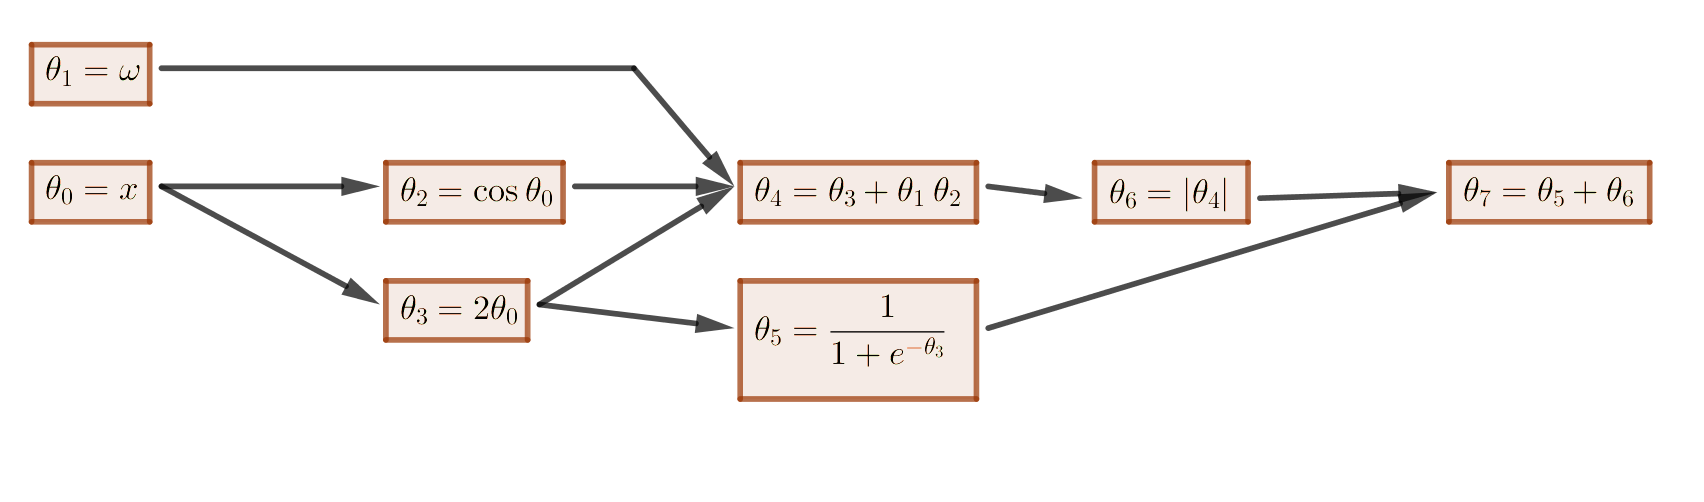
\includegraphics[width=\textwidth]{computation_graph_1}
\caption{A computation graph for the function \(f_\omega(x)=\frac1{1+e^{-2x}}+\left|2x+\omega\cos x\right|.\)}
\label{computation_graph_1}
\end{figure}

We can bound the Lipschitz constant of \(f_\omega\) from above, by upperbounding the partial derivatives of \(\theta_1\), \(\theta_2\), \(\cdots\), \(\theta_7\) consecutively where \(\theta_7=f_\omega(x)\).
%The derivative of \(f_\omega\), and the Lipschitz constant of it can be evaluated consecutively as follows.
%Since, \(\theta_i\) is a function of \(\theta_0\), \(\theta_1\), \(\theta_2\), \(\cdots\), \(\theta_{i-1}\), the partial derivative \$(\frac{\partial\theta_i}{\partial x}\) can be evaluated inductively as follows.
Since \(\theta_1=g_1(\theta_0)=\omega\), we have \(\frac{\partial\theta_1}{\partial x}=0\).
The next parameter \(\theta_2\) is a function of one variable \(\theta_0\), but we regard \(\theta_2\) as a function of two variables ; \(\theta_2=g_2(\theta_0,\theta_1)=\cos\theta_0\).
It is legal to apply the chain rule to get
\begin{align*}
\pa{\theta_2}x
&=\pa{\theta_2}{\theta_0}\pa{\theta_0}x+\pa{\theta_2}{\theta_1}\pa{\theta_1}x\\
&=(-\sin\theta_0)\times1+0\times0\\
&=-\sin x.
\end{align*}
Then, the Lipschitz constant \(\lip(\theta_2)\) of \(\theta_2\) is
\[\norm{\pa{\theta_2}x}=\sup_x|-\sin x|=1.\]
Again, since \(\theta_3=g_3(\theta_0,\theta_1,\theta_2)=2\theta_0\), we have
\begin{align*}
\pa{\theta_3}x
&=\pa{\theta_3}{\theta_0}\pa{\theta_0}x+\pa{\theta_3}{\theta_1}\pa{\theta_1}x+\pa{\theta_3}{\theta_2}\pa{\theta_2}x\\
&=2\times1+0\times0+0\times(-\sin x)=2,
\end{align*}
and thus \(\norm{\pa{\theta_2}x}=2\).
Note that the value of partial derivatives evaluated above, such as \pa{\theta_1}x and \pa{\theta_2}x, can be applied to calcuate \pa{\theta_3}x.
To represent that \norm{\pa{\theta_3}x} is upper bounded by 2, we write \(L_3=2\).
Likewise, let \(L_1=0\) and \(L_0=1\).

For the next parameter \(\theta_4=g_4(\theta_0,\theta_1,\theta_2,\theta_3)=\theta_3+\theta_1\theta_2\), we have
\begin{align*}
\pa{\theta_4}x
&=\pa{\theta_4}{\theta_0}\pa{\theta_0}x+\pa{\theta_4}{\theta_1}\pa{\theta_1}x+\pa{\theta_4}{\theta_2}\pa{\theta_2}x
+\pa{\theta_4}{\theta_3}\pa{\theta_3}x\\
&=0\times1+\theta_2\times0+\theta_1\times(-\sin x)+1\times2\\
\end{align*}
and
\begin{align*}
\norm{\pa{\theta_4}x}
&\le|\omega|\cdot\norm{\pa{\theta_2}x}+1\times\norm{\pa{\theta_3}x}\\
&\le|\omega|\cdot L_2+L_3=|\omega|+2.
\end{align*}
Thus, \(L_4=|\omega|+2\).
%(Here, tighter bound \(|\omega|\) than \(|\omega|+2\) is possible in this case, but we are proposing a genenral upper bound in this section.)

In similar fashions,
\(\theta_5=g_5(\theta_0,\theta_1,\cdots,\theta_4)=\frac1{1+e^{-\theta_3}}\),
\(\theta_6=g_6(\theta_0,\theta_1,\cdots,\theta_5)=|\theta_4|\) and
\(\theta_7=g_7(\theta_0,\theta_1,\cdots,\theta_6)=\theta_5+\theta_6\) have
\begin{align*}
\pa{\theta_5}x&=\pa{\theta_5}{\theta_3}\pa{\theta_3}x&&\norm{\pa{\theta_5}x}\le\frac14\times2=\frac12\\
\pa{\theta_6}x&=\pa{\theta_6}{\theta_4}\pa{\theta_4}x&&\norm{\pa{\theta_6}x}
\le\norm{\pa{\theta_6}{\theta_4}}\norm{\pa{\theta_6}{\theta_4}}=|\omega|+2\\
\pa{\theta_7}x&=\pa{\theta_7}{\theta_5}\pa{\theta_5}x+\pa{\theta_7}{\theta_6}\pa{\theta_6}x&&\norm{\pa{\theta_7}x}
\le\norm{\pa{\theta_5}x}+\norm{\pa{\theta_6}x}\le|\omega|+\frac52.
\end{align*}
Thus, the Lipschitz constant for the function \(f_\omega\) is upper bounded by \(\omega+\frac52\).

%%%
\subsection{AutoLip}
Consider \(f:\mathbb R^n\to\mathbb R^m\), a composite function of elementary functions \(g_0\), \(g_1\), \(g_2\), \(\cdots\), \(g_K\), so that
\[f={g_K}\circ\cdots\circ{g_2}\circ{g_1}\circ{g_0}.\]
For every \(\boldsymbol x\in\mathbb R^n\), define the intermediate variables
\(\theta_0=g_0(\boldsymbol x)\), \(\theta_1=g_1(g_0(\boldsymbol x))\), \(\cdots\), \(\theta_K=g_K(g_{K-1}(\cdots g_1(g_0(\boldsymbol x))))=f(\boldsymbol x)\).
For a notational purpose, let \(g_0\) be the identity function and think of \(g_k\) as a function of \(\theta_0\), \(\theta_1\), \(\cdots\), \(\theta_{k-1}\) for \(1\le k\le K\) and write
%\begin{align*}
%\theta_1&=g_1(\theta_0,\theta_1,\cdots,\theta_{K-1})\\
%\theta_2&=g_2(\theta_0,\theta_1,\cdots,\theta_{K-1})\\
%&\vdots\\
%\theta_K&=g_K(\theta_0,\theta_1,\cdots,\theta_{K-1}).
%\end{align*}
\begin{align*}
\theta_1&=g_1(\theta_0)\\
\theta_2&=g_2(\theta_0,\theta_1)\\
&\vdots\\
\theta_K&=g_K(\theta_0,\theta_1,\cdots,\theta_{K-1}).
\end{align*}
An upper bound \(L_k\) for the lipschitz constant \(\sup_{\boldsymbol x}\left|\left|\frac{\partial\theta_k}{\partial\boldsymbol x}\right|\right|\) of \(\theta_k\), can be evaulated inductively, where \(L_K\) is an upper bound for \(\lip(f)\).

Let \(L_0=1\).
Suppose that suppose that \(k\) is an integer such that \(1\le k\le K\) and we have an upper bound \(L_i\) of the Lipschitz constant
\[\sup_{\boldsymbol x}\left|\left|\frac{\partial\theta_i}{\partial\boldsymbol x}\right|\right|\le L_i\]
for \(1\le i\le k-1\).
Since
\begin{align*}
\frac{\partial \theta_k}{\partial\boldsymbol x}
&=\frac{\partial\theta_k}{\partial\theta_0}\frac{\partial\theta_0}{\partial\boldsymbol x}
+\frac{\partial\theta_k}{\partial\theta_1}\frac{\partial\theta_1}{\partial\boldsymbol x}
+\cdots
+\frac{\partial\theta_k}{\partial\theta_{k-1}}\frac{\partial\theta_{k-1}}{\partial\boldsymbol x}\\
&=\sum_{i=0}^{k-1}\frac{\partial\theta_k}{\partial\theta_i}\frac{\partial\theta_i}{\partial\boldsymbol x},
\end{align*}
it follows that
\begin{align*}
\left|\left|\frac{\partial \theta_k}{\partial\boldsymbol x}\right|\right|
&\le\sum_{i=0}^{k-1}
\left|\left|\frac{\partial\theta_k}{\partial\theta_i}\right|\right|
\left|\left|\frac{\partial\theta_i}{\partial\boldsymbol x}\right|\right|
\end{align*}
and that
\begin{align*}
\sup_{\boldsymbol x}\left|\left|\frac{\partial \theta_k}{\partial\boldsymbol x}\right|\right|
&\le\sum_{i=0}^{k-1}
\sup\left|\left|\frac{\partial\theta_k}{\partial\theta_i}\right|\right|\cdot L_i.
\end{align*}
Let \(L_k\) be the right hand side of the above inequality and proceed for \(k+1\).
After \(K\) iterations, we have an upper bound \(L_K\) of the lipschitz constant for \(\theta_K=f(\boldsymbol x)\).
(\textbf{Algorithm} \ref{alg:1})

\begin{algorithm}
\SetKwInOut{Input}{input}\SetKwInOut{Output}{output}
\Input{the function \(f=g_K\circ\cdots\circ g_0\), where \(\theta_k=(g_k\circ\cdots\circ g_0)(\boldsymbol x)\) for \(0\le k\le K\).}
\Output{An upper bound \(L\) for \(\lip(f)\)}
\BlankLine
\(k\gets 0\)\;
\(L_0\gets1\)\;
\While{\(k<K\)}{
\(L_k\gets\sum_{i=0}^{k-1}\left(\sup\left|\left|\frac{\partial\theta_k}{\partial\theta_i}\right|\right|\right)L_i\)\;
\(k\gets k+1\)\;
}
\(L\gets L_K\)
\caption{AutoLip}
\label{alg:1}
\end{algorithm}

%%
\section{Multi-Layer Perceptrons}
Consider a single layer perceptron (Figure \ref{SLP}).
Denote the single layer perceptron by \(f_\omega:\mathbb R^3\to\mathbb R^4\), which is defined as
\[f_\omega(\bx)=\text{ReLU}(W\bx+b),\]
where \(\omega\) stands for the set of parameters : \(\omega=(W,b)\).
With the computation graph illustrated in Figure \ref{computation_graph_2}, we have

\begin{figure}[h]
\centering
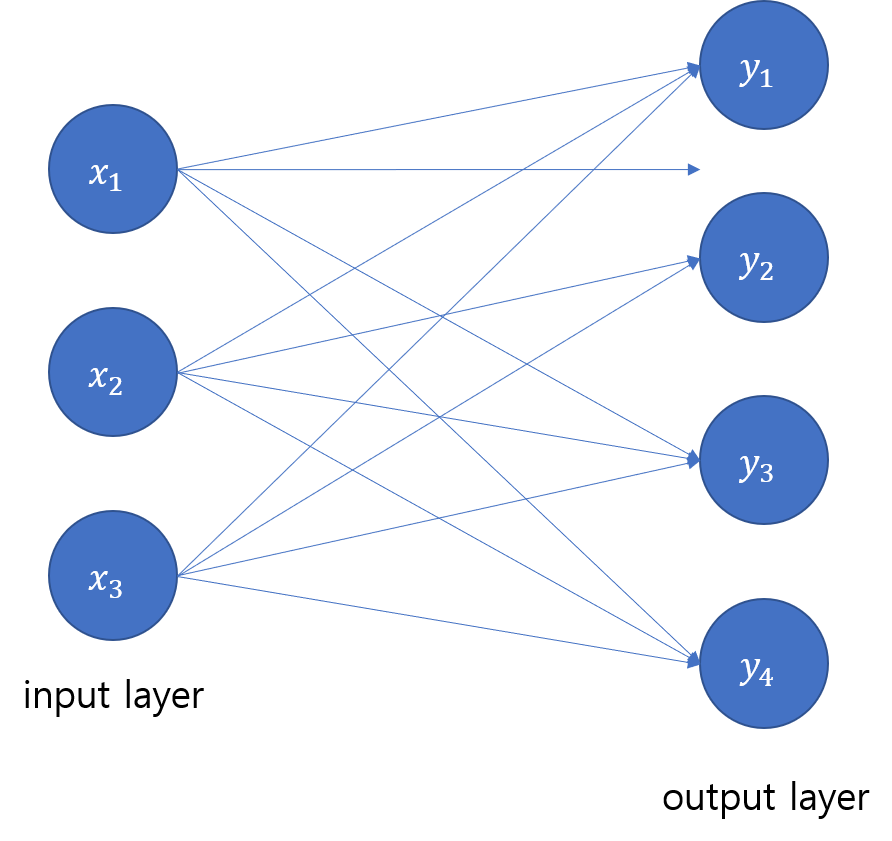
\includegraphics[width=.4\textwidth]{SLP}
\caption{A single layer perceptron of input dimension 3 and output dimension 4 with weight matrix \(W\) and the bias \(b\).}
\label{SLP}
\end{figure}

\begin{figure}[h]
\centering
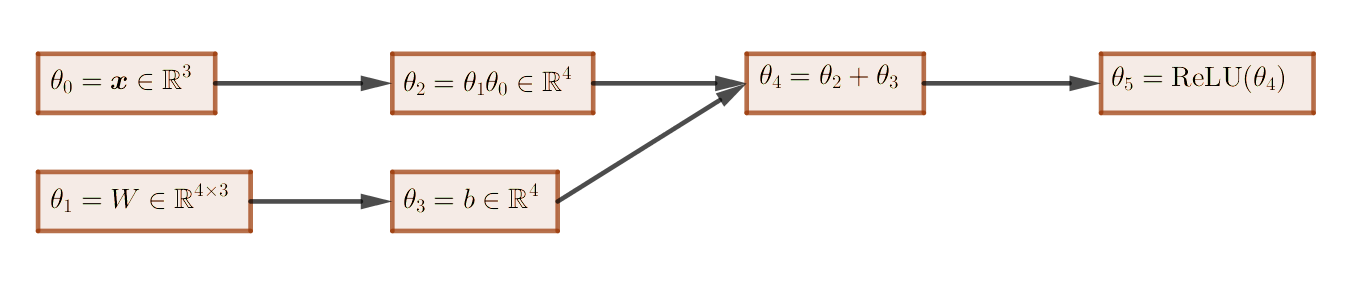
\includegraphics[width=\textwidth]{computation_graph_2}
\caption{A computation graph for a single layer perceptron}
\label{computation_graph_2}
\end{figure}

\begin{align*}
k=0;\:\: L_0&=1\\
k=1;\:\: L_1&=\sup\norm{\frac{\partial\theta_1}{\partial\theta_0}}\times L_0=0\times1=0\\
k=2;\:\: L_2&
=\sup\norm{\frac{\partial\theta_2}{\partial\theta_0}}\times L_0
+\sup\norm{\frac{\partial\theta_2}{\partial\theta_1}}\times L_1\\
&=||W||\times1+||\bx||\times0=||W||\\
k=3;\:\: L_3&
=\sup\norm{\frac{\partial\theta_3}{\partial\theta_0}}\times L_0
+\sup\norm{\frac{\partial\theta_3}{\partial\theta_1}}\times L_1
+\sup\norm{\frac{\partial\theta_3}{\partial\theta_2}}\times L_2=0\\
k=4;\:\: L_4&
=\sup\norm{\frac{\partial\theta_4}{\partial\theta_0}}\times L_0
+\sup\norm{\frac{\partial\theta_4}{\partial\theta_1}}\times L_1
+\sup\norm{\frac{\partial\theta_4}{\partial\theta_2}}\times L_2
+\sup\norm{\frac{\partial\theta_4}{\partial\theta_3}}\times L_3\\
&=0\times1+0\times0+1\times||W||+1\times0=||W||\\
k=5;\:\: L_5&
=\sup\norm{\frac{\partial\theta_5}{\partial\theta_0}}\times L_0
+\sup\norm{\frac{\partial\theta_5}{\partial\theta_1}}\times L_1
+\sup\norm{\frac{\partial\theta_5}{\partial\theta_2}}\times L_2
+\sup\norm{\frac{\partial\theta_5}{\partial\theta_3}}\times L_3
+\sup\norm{\frac{\partial\theta_5}{\partial\theta_4}}\times L_4\\
&=0\times1+0\times0+0\times||W||+0\times0+1\times||W||=||W||.
\end{align*}
The resulting upper bound for the Lipschitz constant is \(||W||\).
Note that we've used the fact that \(\lip(\text{ReLU})=1\).

Let \(f\) be a multi layer perceptron of \(N\) layers, with 1-Lipschitz activation functions (like ReLU, Leaky ReLU, \(\tanh\), or SoftPlus).
Then, we can think of \(f\) as a composite of \(f_1\), \(f_2\), \(\cdots\), \(f_N\) where each \(f_i\) is a single layer perceptron described in the above paragraph, for \(1\le n\le N\).
Then,
\[\lip(f)\le\prod_{i=1}^n\lip(f_n)\le\prod_{i=1}^n||W_n||,\]
where each \(W_n\) is a weight matrix in the \(n\)th layer.

%%
\section{Convolutional Neural Networks}

A vanilla convolutional neural network is a composition of convolutional layers, max pooling layers and linear layers.
VGG-16, for example, consists of 13 convolutional layers, 5 maxpooling layers, 3 fully connected layers and a softmax function in the output layer \cite{SK-ZA}.
While linear layers are what we've discussed in the previous section, we need to evaluate the Lipschitz constant of convolutional layers and max pooling layers.

%%%
\subsection{Convolutional layers}\label{convolutional_layers}
Consider a convolutional layer of \(5\times 5\) input array and \(3\times 3\) filters.
To make it simple, suppose that it has only one channel and that padding option is set to \texttt{valid} so that the output array is of \(3\times 3\).
Denote the input array, the filter and the output array by \(X\), \(F\) and \(Y\).
Instead of viewing \(X\) and \(Y\) as matrices(e.g. \(X=[x_{ij}]_{5\times 5}\), \(Y=[y_{ij}]_{3\times 3}\)), let \(X\) and \(Y\) be column vectors of dimension \(25\) and \(9\), respectively, so that
%Let \(X=(x_{ij})_{6\times 6}\), \(F=(f_{ij})_{3\times 3}\), \(Y=(y_{ij})_{4\times 4}\) be matrix for
\[X=\begin{bmatrix}x_{11}\\x_{12}\\\vdots\\x_{55}\end{bmatrix},\quad
Y=\begin{bmatrix}y_{11}\\y_{12}\\\vdots\\y_{33}\end{bmatrix}.\]
Then, we can think of the convolutional layer as left multiplication of a matrix \(F\) (Figure \ref{convolution_matrix}).

%The matrix \(F\) in general, is a sparse matrix which is wide ; the number of columns are far larger than the number of rows.
The Lipschitz constant for the convolution layer is, thus, the operator norm of the matrix \(F\) and we can use the Theorem \ref{theo:evaluation_for_rectangular_matrices}.

%Although \(F\) is big and wide, the computation of \(||F||\) is not that hard.
%Let \(f_i\) be the vector of dimension \(3\) defined by
%\(f_i=[f_{i1}\:\:f_{i2}\:\:f_{i3}]^T\)
%%\(f_i=\begin{bmatrix}f_{i1}&f_{i2}&f_{i3}\end{bmatrix}\)
%for \(i=1,2,3\);
%\begin{align*}
%f_1&=[f_{11}\:\:f_{12}\:\:f_{13}]^T\\
%f_2&=[f_{21}\:\:f_{22}\:\:f_{23}]^T\\
%f_3&=[f_{31}\:\:f_{32}\:\:f_{33}]^T
%\end{align*}
%The \(9\times9\) square matrix \(FF^T\) is of the form

\begin{figure}[h]
\centering
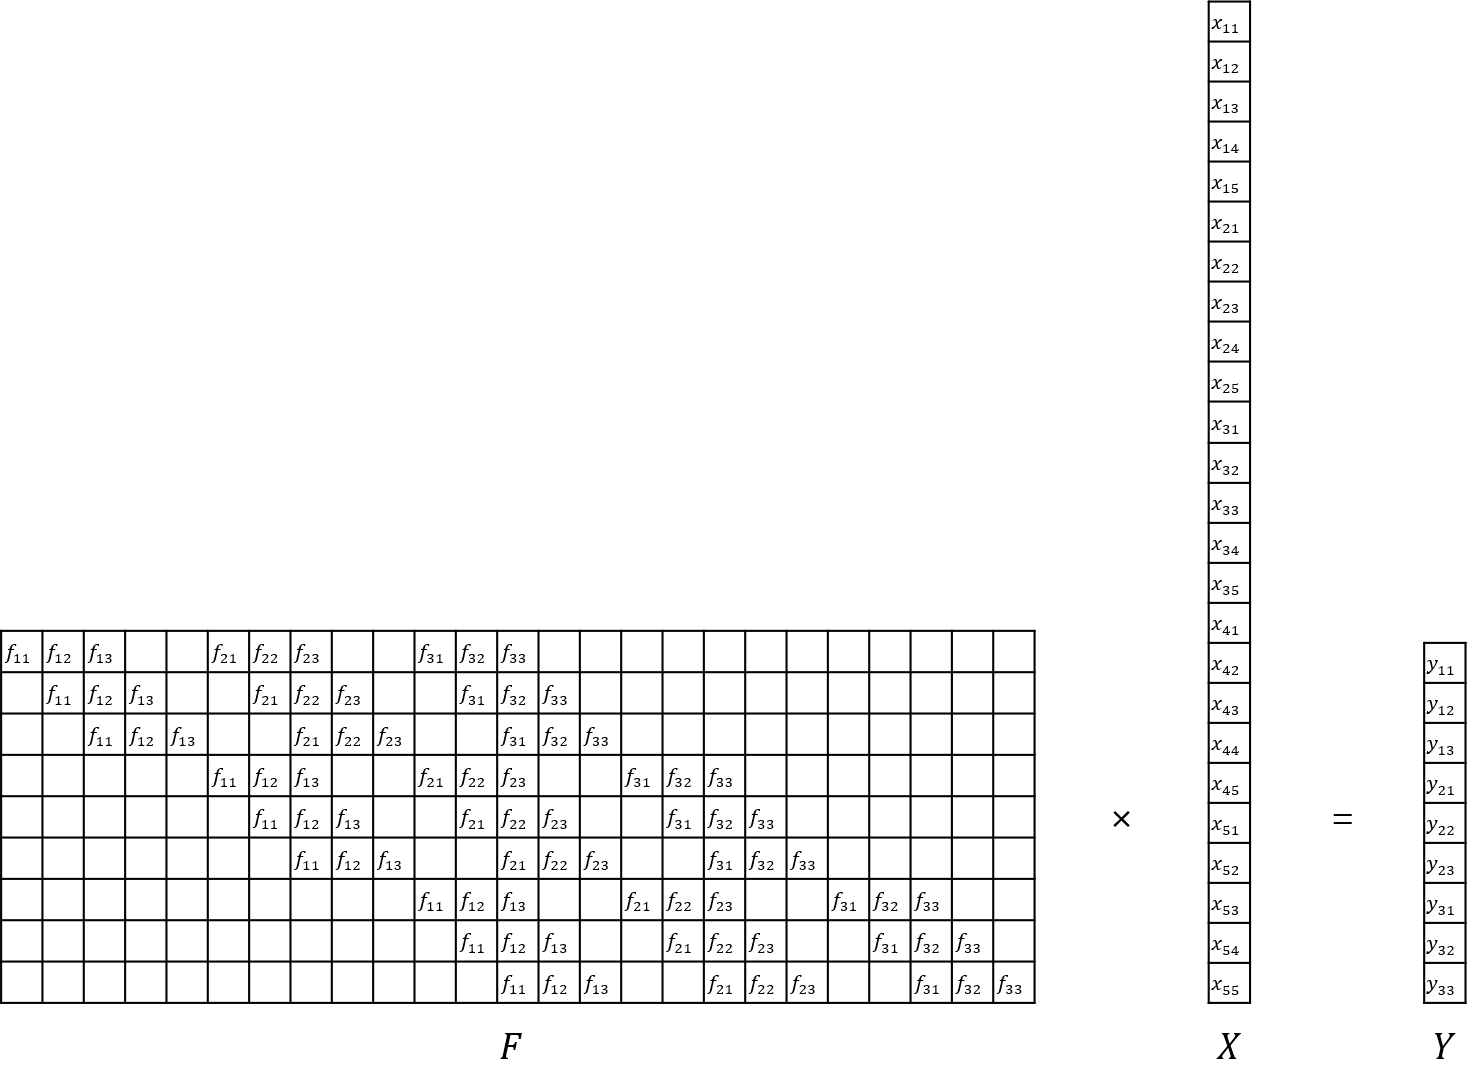
\includegraphics[width=\textwidth]{convolution_matrix}
\caption{A convolutional layer as a matrix multiplication}
\label{convolution_matrix}
\end{figure}

But, it is complicated and time consuming to evaluate the Lipschitz constant directly.
Instead of applying the Theorem \ref{theo:evaluation_for_rectangular_matrices} and evaluate \(||F||=\sqrt{||F^TF||}\) rigorously, we can use numerical method called \emph{power method}.

%%%
\subsection{Power method}\label{sec:power_method}
Supposet that \(A\in\mathbb R^{n\times n}\) is an orthogonally diagonalizable matrix, or that \(A\) has distinct eigenvalues \(\lambda_1\), \(\lambda_2\), \(\cdots\), \(\lambda_n\).
This is usually the case, since the probability that the characteristic equation happen to have repeated root is 0.

Then, we have not only the distinct eigenvalues \(\lambda_1\), \(\cdots\), \(\lambda_n\), but also the linearly independent eigenvectors \(v_1\), \(\cdots\), \(v_n\).
Without loss of generality, let \(|\lambda_1|\ge|\lambda_2|\ge\cdots\ge|\lambda_n|\), so that \(\lambda_1\) is the \emph{dominating eigenvalue} ; \(|\lambda_1|=\max_i|\lambda_i|\).

Let \(x\) be any nonzero vector in \(\mathbb R^n\).
There exist \(c_1\), \(\cdots\), \(c_n\) such that
\[x=c_1v_1+\cdots+c_nv_n.\]
Then,
\begin{align*}
Ax
&=A(c_1v_1+\cdots+c_nv_n)\\
&=c_1Av_1+\cdots+c_nAv_n\\
&=c_1\lambda_1v_1+\cdots+c_n\lambda_nv_n.
\end{align*}
Moreover,
\begin{align*}
A^2x
&=A(c_1\lambda_1v_1+\cdots+c_n\lambda_nv_n)\\
&=c_1\lambda_1Av_1+\cdots+c_n\lambda_nAv_n\\
&=c_1{\lambda_1}^2v_1+\cdots+c_n{\lambda_n}^2v_n.
\end{align*}
In the similar fashion, we have, for any positive integer \(k\),
\[A^kx=c_1{\lambda_1}^kv_1+\cdots+c_n{\lambda_n}^kv_n.\]
Among \(n\) terms \(c_1{\lambda_1}^kv_1\), \(\cdots\), \(c_n{\lambda_n}^kv_n\), the first term is the dominating term, since
\[A^kx={\lambda_1}^k\left(c_1v_1+c_2\left(\frac{\lambda_2}{\lambda_1}\right)^kv_2+\cdots+c_n\left(\frac{\lambda_n}{\lambda_1}\right)^kv_n\right)\]
and
\(\left(\frac{\lambda_i}{\lambda_1}\right)^k\to0\) exponentially as \(k\to\infty\), for \(i=2,\cdots,n\).
In short, for sufficient large integer \(k\), we have
\[A^kx\approx c_1{\lambda_1}^kv_1.\]
Furthermore, we can approximately think of \(A^kx\) as the eigenvector, corresponding eigenvalue of which is the dominating one.
Now, we can use the following lemma, stating that if we are given an eigenvector, we can evaluate the the corresponding eigenvalue.

\begin{lemma}\label{lemm:Rayleigh}
\textbf{(Rayleigh Quotient)}
If \(x\) is an eigenvector of a matrix \(A\), then its corresponding eigenvalue is given by
\[\lambda = \frac{\langle Ax,x\rangle}{\langle x,x\rangle}.\]
\end{lemma}
Here, \(\langle\cdot,\cdot\rangle\) is the inner product as defined in Subsection \ref{sec:evaluation_for_rectangular_matrices}.

Therefore, given a square orthogonally diagonalizable matrix $A$, we can approximate the \emph{dominating eigenvector} $x_1$, by computing repeatedly $A^kx$ for any nonzero vector $x$, and also the corresponding \emph{dominating eigenvalue} $\lambda_1$ by the above lemma, which converges to $||A||$.
For rectangular matrix \(f\), for example, as in Subsection \ref{convolutional_layers}, approximating algorithm for \(||F||\) is illustrated in \textbf{Algorithm} \ref{alg:2}.

%Therefore, the dominating eigenvalue \(\tilde\lambda\) of a square matrix \(A\) or the operator norm of \(A\) can be approximated by
%\[\tilde\lambda\approx\frac{\langle A^{k+1}x,A^kx\rangle}{\langle A^kx,A^kx\rangle}.\]


\begin{algorithm}
\SetKwInOut{Input}{input}\SetKwInOut{Output}{output}
\Input{A rectangular matrix \(F\in\mathbb R^{n\times m}\).}
\Output{Approximation for \(||F||\)}
\BlankLine
\(A\gets F^TF\)\;
Set an integer \(k\) sufficiently large enough\;
Set a nonzero vector \(x\in\mathbb R^m\)\;
\(x_k\gets A^kx\)\;
\(\tilde\lambda\gets\frac{{x_k}^TAx_k}{{x_k}^Tx_k}\)\;
\(||F||\gets\sqrt{\tilde\lambda}\)
\caption{Approximating \(||F||\) using the power method}
\label{alg:2}
\end{algorithm}

%%%
\subsection{Max pooling layers}

The Lipschitz constant of the max pooling component is 1, by the following obvious reason.

Consider a usual \(2\times 2\) maxpooling, applied to 2d-array \(X\).
Suppose that \(X\) consists \(4N\) numbers \(x_1\), \(x_2\), \(x_3\), \(x_4\), \(\cdots\), \(x_{4N-3}\), \(x_{4N-2}\), \(x_{4N-1}\), \(x_{4N}\) and denote \(X\) as a \(4N\)-dimensional vector by
\[X=[x_1\:\:\:x_2\:\:\:x_3\:\:\:x_4\:\:\:\cdots\:\:\:x_{4N-3}\:\:\:x_{4N-2}\:\:\:x_{4N-1}\:\:\:x_{4N}]^T.\]
Let \(x^{(1)}\), \(\cdots\), \(x^{(N)}\) be four dimensional vectors defined by
\[x^{(1)}=\begin{bmatrix}x_1\\x_2\\x_3\\x_4\end{bmatrix},\cdots,x^{(N)}=\begin{bmatrix}x_{4N-3}\\x_{4N-2}\\x_{4N-1}\\x_{4N}\end{bmatrix}\]
and write
\[X=\begin{bmatrix}x^{(1)}\\\vdots\\x^{(N)}\end{bmatrix}.\]
%by abusing notation.

\begin{lemma}\label{lemm:maxs_1_lipschitz}
A function \([a_1,\:a_2\:a_3,\:a_4]^T\mapsto\max a_i\) is 1-Lipschitz function.
\end{lemma}
\begin{proof}
Denote \(a=[a_1,\:a_2\:a_3,\:a_4]^T\) and \(b=[b_1,\:b_2\:b_3,\:b_4]^T\).
Let \(a_{i_0}=\max a_i\).
Then,
\[\max a_i-\max b_i=a_{i_0}-\max b_i\le a_{i_0}-b_{i_0}\le\max (a_i-b_i).\]
Similarly, \[\max b_i-\max a_i\le\max (a_i-b_i).\]
Thus,
\[\left|\max a_i-\max b_i\right|\le\max (a_i-b_i),\]
and \(\lip(\max)=1\).
\end{proof}

Now, we are ready to evaluate \(\lip(\text{MaxPool})\).
The function \[\text{MaxPool}:\mathbb R^{4N}\to\mathbb R^N\] is defined by
\[\text{MaxPool}(X)=\begin{bmatrix}\max \left(x^{(1)}\right)\\\vdots\\\max \left(x^{(N)}\right)\end{bmatrix}.\]
Thus,
\begin{align*}
{\left|\left|\text{MaxPool}(X)-\text{MaxPool}(Y)\right|\right|_2}^2
&=\sum_{n=1}^N\left(\max\left(x^{(n)}\right)-\max\left(y^{(n)}\right)\right)^2\\
&\le\sum_{n=1}^N\left(\max\left(x^{(n)}-y^{(n)}\right)\right)^2\\
&{\le\left|\left|\text{MaxPool}(X-Y)\right|\right|_2}^2.
\end{align*}
Therefore,
\[\lip(\text{MaxPool})=1.\]
%\[m(x_1,\cdots,x_n)=\max(x_1,\cdots,x_n)\]
%has \(\lip(m)=1\).

%%%
\chapter{Conclusion}
For a function between metric spaces, the Lipschitz constant measures the rate of change of the function.
If we conceive a neural network as a function between Euclidean spaces, the Lipschitz constant of the neural network tells us how sensitive the output is, relative to the input.
One can relate the Lipschitz constant to the robustness of the algorithm.
But the Lipschitz constant is not the same as the robustness of an \emph{architecture}, in that it measures the sensitivity of an \emph{algorithm} when the parameters are fixed.
We may further study the robustness by investigating the changes of the Lipschitz constant when updating the parameters of the algorithm.

The Lipscthiz constant for relatively simple functions such as activation functions, linear functions and affine functions can be obtained either by simple calculation or the notion of matrix norm.
We can express the Lipschitz constant of \emph{any} locally Lipschitz functions by Rademacher Theorem, but evaluating the optimal constant in its exact value is difficult or not feasible.
Rather, we can think of several numerical way to find an upper bound for the optimal constant either by an algorithm called AutoLip or by the Rayleigh quotient and power method.
This paper doesn't include the implementation with programming code, such as Python.
One may relate the calculations to the experimental results.

%%% Reference(or Bibliography)
\newpage
\renewcommand\bibname{Reference}
\addcontentsline{toc}{chapter}{Bibliography}
\begin{thebibliography}{AA}
\bibitem {VA-SK} Virmaux, A., \& Scaman, K. (2018). Lipschitz regularity of deep neural networks: analysis and efficient estimation.
\emph{Advances in Neural Information Processing Systems}, 31.
\bibitem {CS-WZ} Szegedy, C., Zaremba, W., Sutskever, I., Bruna, J., Erhan, D., Goodfellow, I., \& Fergus, R. (2014). Intriguing properties of neural networks. \emph{Proceedings of the International Conference on Learning Representations (ICLR)}
\bibitem {MA-SC} Arjovsky, M., Chintala, S., \& Bottou, L. (2017, July). Wasserstein generative adversarial networks. In International conference on machine learning (pp. 214-223). PMLR.
\bibitem {GI-AF} Gulrajani, I., Ahmed, F., Arjovsky, M., Dumoulin, V., \& Courville, A. C. (2017). Improved training of wasserstein gans. Advances in neural information processing systems, 30.
\bibitem {KC} Computing The Norm of a matrix, \url{https://kconrad.math.uconn.edu/blurbs/linmultialg/matrixnorm.pdf}, University of Connecticut.
\bibitem {IG-YB}Goodfellow, I., Bengio, Y., \& Courville, A. (2016). Deep learning. MIT press.
\bibitem {WR} Rudin, Walter. \emph{Real and Complex Analysis.} : McGraw-Hill Science/Engineering/Math, 1986.
\bibitem {HF} Herbert Federer. \emph{Geometric measure theory.} Classics in Mathematics. Springer-Verlag Berlin Heidelberg, 1969.
\bibitem {VC} Villani, C. (2009). \emph{Optimal transport: old and new} (Vol. 338, p. 23). Berlin: springer.
\bibitem {PH} Piotr Hajłasz, \emph{Geometric Analysis}, \url{https://sites.pitt.edu/~hajlasz/Teaching/Math2304Spring2014/Part\%201.pdf}, University of Pittsburgh.
\bibitem {JM} James T. Murphy, \emph{An elementary proof of Rademacher's theorem}, \url{https://intfxdx.com/downloads/rademacher-thm-2015.pdf}
THEOREM
\bibitem {JM-DA} Jordan, M., \& Dimakis, A. G. (2020). Exactly computing the local lipschitz constant of relu networks. \emph{Advances in Neural Information Processing Systems}, 33, 7344-7353.
\bibitem {BA-DS} Bhowmick, A., D’Souza, M., \& Raghavan, G. S. (2021, September). Lipbab: computing exact lipschitz constant of relu networks. \emph{In International Conference on Artificial Neural Networks} (pp. 151-162). Springer, Cham.
\bibitem {BG-HM} Beer, G., \& Hoffman, M. J. (2013). The Lipschitz metric for real-valued continuous functions. \emph{Journal of Mathematical Analysis and Applications}, 406(1), 229-236.
\bibitem {CN-WD} Carlini, N., \& Wagner, D. (2017, May). Towards evaluating the robustness of neural networks. In 2017 \emph{ieee symposium on security and privacy (sp)} (pp. 39-57). Ieee.
\bibitem {SK-ZA} Simonyan, K., \& Zisserman, A. (2014). Very deep convolutional networks for large-scale image recognition. arXiv preprint arXiv:1409.1556.

\end{thebibliography}

%%% the appendix chapters : 생략

\end{document}